% Options for packages loaded elsewhere
\PassOptionsToPackage{unicode}{hyperref}
\PassOptionsToPackage{hyphens}{url}
%
\documentclass[
]{article}
\title{Workshop Notes}
\author{Dan Tran}
\date{2022-09-20}

\usepackage{amsmath,amssymb}
\usepackage{lmodern}
\usepackage{iftex}
\ifPDFTeX
  \usepackage[T1]{fontenc}
  \usepackage[utf8]{inputenc}
  \usepackage{textcomp} % provide euro and other symbols
\else % if luatex or xetex
  \usepackage{unicode-math}
  \defaultfontfeatures{Scale=MatchLowercase}
  \defaultfontfeatures[\rmfamily]{Ligatures=TeX,Scale=1}
\fi
% Use upquote if available, for straight quotes in verbatim environments
\IfFileExists{upquote.sty}{\usepackage{upquote}}{}
\IfFileExists{microtype.sty}{% use microtype if available
  \usepackage[]{microtype}
  \UseMicrotypeSet[protrusion]{basicmath} % disable protrusion for tt fonts
}{}
\makeatletter
\@ifundefined{KOMAClassName}{% if non-KOMA class
  \IfFileExists{parskip.sty}{%
    \usepackage{parskip}
  }{% else
    \setlength{\parindent}{0pt}
    \setlength{\parskip}{6pt plus 2pt minus 1pt}}
}{% if KOMA class
  \KOMAoptions{parskip=half}}
\makeatother
\usepackage{xcolor}
\IfFileExists{xurl.sty}{\usepackage{xurl}}{} % add URL line breaks if available
\IfFileExists{bookmark.sty}{\usepackage{bookmark}}{\usepackage{hyperref}}
\hypersetup{
  pdftitle={Workshop Notes},
  pdfauthor={Dan Tran},
  hidelinks,
  pdfcreator={LaTeX via pandoc}}
\urlstyle{same} % disable monospaced font for URLs
\usepackage[margin=1in]{geometry}
\usepackage{color}
\usepackage{fancyvrb}
\newcommand{\VerbBar}{|}
\newcommand{\VERB}{\Verb[commandchars=\\\{\}]}
\DefineVerbatimEnvironment{Highlighting}{Verbatim}{commandchars=\\\{\}}
% Add ',fontsize=\small' for more characters per line
\usepackage{framed}
\definecolor{shadecolor}{RGB}{48,48,48}
\newenvironment{Shaded}{\begin{snugshade}}{\end{snugshade}}
\newcommand{\AlertTok}[1]{\textcolor[rgb]{1.00,0.81,0.69}{#1}}
\newcommand{\AnnotationTok}[1]{\textcolor[rgb]{0.50,0.62,0.50}{\textbf{#1}}}
\newcommand{\AttributeTok}[1]{\textcolor[rgb]{0.80,0.80,0.80}{#1}}
\newcommand{\BaseNTok}[1]{\textcolor[rgb]{0.86,0.64,0.64}{#1}}
\newcommand{\BuiltInTok}[1]{\textcolor[rgb]{0.80,0.80,0.80}{#1}}
\newcommand{\CharTok}[1]{\textcolor[rgb]{0.86,0.64,0.64}{#1}}
\newcommand{\CommentTok}[1]{\textcolor[rgb]{0.50,0.62,0.50}{#1}}
\newcommand{\CommentVarTok}[1]{\textcolor[rgb]{0.50,0.62,0.50}{\textbf{#1}}}
\newcommand{\ConstantTok}[1]{\textcolor[rgb]{0.86,0.64,0.64}{\textbf{#1}}}
\newcommand{\ControlFlowTok}[1]{\textcolor[rgb]{0.94,0.87,0.69}{#1}}
\newcommand{\DataTypeTok}[1]{\textcolor[rgb]{0.87,0.87,0.75}{#1}}
\newcommand{\DecValTok}[1]{\textcolor[rgb]{0.86,0.86,0.80}{#1}}
\newcommand{\DocumentationTok}[1]{\textcolor[rgb]{0.50,0.62,0.50}{#1}}
\newcommand{\ErrorTok}[1]{\textcolor[rgb]{0.76,0.75,0.62}{#1}}
\newcommand{\ExtensionTok}[1]{\textcolor[rgb]{0.80,0.80,0.80}{#1}}
\newcommand{\FloatTok}[1]{\textcolor[rgb]{0.75,0.75,0.82}{#1}}
\newcommand{\FunctionTok}[1]{\textcolor[rgb]{0.94,0.94,0.56}{#1}}
\newcommand{\ImportTok}[1]{\textcolor[rgb]{0.80,0.80,0.80}{#1}}
\newcommand{\InformationTok}[1]{\textcolor[rgb]{0.50,0.62,0.50}{\textbf{#1}}}
\newcommand{\KeywordTok}[1]{\textcolor[rgb]{0.94,0.87,0.69}{#1}}
\newcommand{\NormalTok}[1]{\textcolor[rgb]{0.80,0.80,0.80}{#1}}
\newcommand{\OperatorTok}[1]{\textcolor[rgb]{0.94,0.94,0.82}{#1}}
\newcommand{\OtherTok}[1]{\textcolor[rgb]{0.94,0.94,0.56}{#1}}
\newcommand{\PreprocessorTok}[1]{\textcolor[rgb]{1.00,0.81,0.69}{\textbf{#1}}}
\newcommand{\RegionMarkerTok}[1]{\textcolor[rgb]{0.80,0.80,0.80}{#1}}
\newcommand{\SpecialCharTok}[1]{\textcolor[rgb]{0.86,0.64,0.64}{#1}}
\newcommand{\SpecialStringTok}[1]{\textcolor[rgb]{0.80,0.58,0.58}{#1}}
\newcommand{\StringTok}[1]{\textcolor[rgb]{0.80,0.58,0.58}{#1}}
\newcommand{\VariableTok}[1]{\textcolor[rgb]{0.80,0.80,0.80}{#1}}
\newcommand{\VerbatimStringTok}[1]{\textcolor[rgb]{0.80,0.58,0.58}{#1}}
\newcommand{\WarningTok}[1]{\textcolor[rgb]{0.50,0.62,0.50}{\textbf{#1}}}
\usepackage{longtable,booktabs,array}
\usepackage{calc} % for calculating minipage widths
% Correct order of tables after \paragraph or \subparagraph
\usepackage{etoolbox}
\makeatletter
\patchcmd\longtable{\par}{\if@noskipsec\mbox{}\fi\par}{}{}
\makeatother
% Allow footnotes in longtable head/foot
\IfFileExists{footnotehyper.sty}{\usepackage{footnotehyper}}{\usepackage{footnote}}
\makesavenoteenv{longtable}
\usepackage{graphicx}
\makeatletter
\def\maxwidth{\ifdim\Gin@nat@width>\linewidth\linewidth\else\Gin@nat@width\fi}
\def\maxheight{\ifdim\Gin@nat@height>\textheight\textheight\else\Gin@nat@height\fi}
\makeatother
% Scale images if necessary, so that they will not overflow the page
% margins by default, and it is still possible to overwrite the defaults
% using explicit options in \includegraphics[width, height, ...]{}
\setkeys{Gin}{width=\maxwidth,height=\maxheight,keepaspectratio}
% Set default figure placement to htbp
\makeatletter
\def\fps@figure{htbp}
\makeatother
\setlength{\emergencystretch}{3em} % prevent overfull lines
\providecommand{\tightlist}{%
  \setlength{\itemsep}{0pt}\setlength{\parskip}{0pt}}
\setcounter{secnumdepth}{-\maxdimen} % remove section numbering
\usepackage{booktabs}
\usepackage{longtable}
\usepackage{array}
\usepackage{multirow}
\usepackage{wrapfig}
\usepackage{float}
\usepackage{colortbl}
\usepackage{pdflscape}
\usepackage{tabu}
\usepackage{threeparttable}
\usepackage{threeparttablex}
\usepackage[normalem]{ulem}
\usepackage{makecell}
\usepackage{xcolor}
\ifLuaTeX
  \usepackage{selnolig}  % disable illegal ligatures
\fi

\begin{document}
\maketitle

{
\setcounter{tocdepth}{3}
\tableofcontents
}
Workshop Recordings can be found on the Learning Resources Site:
\url{https://blackboard.qut.edu.au/bbcswebdav/pid-1481644-dt-announcement-rid-58665563_1/courses/MXB107_22se2/_site/videos.html}.

In this document, I'll only write things that are not included in the
official Workshop resources (above).

\hypertarget{workshop-4-23822}{%
\subsection{Workshop 4 (23/8/22)}\label{workshop-4-23822}}

\hypertarget{largest-dice-roll}{%
\subsubsection{Largest Dice Roll}\label{largest-dice-roll}}

Imagine everyone in this class is lost in a far-away desert. There is
not enough food, so we decide who get to eat by rolling two dices.

Team A would win if the largest face rolled between the two is 1,2,3 or
4.

Team B win otherwise (if the largest face is 5 or 6).

Let \(A\) be the event that team A win, and \(B\) the event that team B
win.

\begin{longtable}[]{@{}lllllll@{}}
\toprule
& 1 & 2 & 3 & 4 & 5 & 6 \\
\midrule
\endhead
\textbf{1} & A & A & A & A & B & B \\
\textbf{2} & A & A & A & A & B & B \\
\textbf{3} & A & A & A & A & B & B \\
\textbf{4} & A & A & A & A & B & B \\
\textbf{5} & B & B & B & B & B & B \\
\textbf{6} & B & B & B & B & B & B \\
\bottomrule
\end{longtable}

By counting, we observe that:

\[
\begin{aligned}
Pr(A) &= \dfrac{16}{36} \approx 44.4\% \\
Pr(B) &= \dfrac{20}{36} \approx 55.6\%
\end{aligned}
\] We see that team B actually wins more often than team A.

\hypertarget{bayesian-rare-disease}{%
\subsubsection{Bayesian: Rare Disease}\label{bayesian-rare-disease}}

There is a rare yet deadly disease that affects 0.1\% of the population.
To diagnose the disease, scientists have made a test kit with 99\%
accuracy. This is, if the patient indeed has the disease, it will test
positive 99\% of the time (and if you are sick, there is a 1\% chance
that it says negative). This also means that even if you are not sick,
it can give positive result 1\% of the time.

\hypertarget{positive-once}{%
\paragraph{Positive Once}\label{positive-once}}

What is the probability that you have the disease given that you tested
positive once?

\textbf{Answer}

Let \(S\) be the event that you are sick, and \(P\) be the event that
you test positive.

\[
\begin{aligned}
Pr(S) &= 0.001 \\
Pr(P | S) &= 0.99 \\
Pr(P | S^c) &= 0.01 \\
Pr(P^c |S) &= 0.01
\end{aligned}
\] We need to find \(Pr(S|P)\), Bayesian Theorem would state that:

\[
\begin{aligned}
Pr(S|P) &= \dfrac{Pr(P|S)Pr(S)}{Pr(P)} \\
Pr(P) &= Pr(P|S)Pr(S) + Pr(P|S^c)Pr(S^c) & (\text{Law of total probability}) \\
\\ \text{Substitution:} \\
\Rightarrow Pr(S|P) &= \dfrac{Pr(P|S)Pr(S)}{Pr(P|S)Pr(S) + Pr(P|S^c)Pr(S^c)} \\
&= \dfrac{0.99\times0.001}{0.99\times 0.001 + 0.01\times0.999} \\
&\approx 0.0901\approx9.01\%
\end{aligned}
\] Hence, if you tested positive once, the probability that you actually
have the disease is 9.01\% (which is not that bad!).

\hypertarget{positive-twice}{%
\paragraph{Positive Twice*}\label{positive-twice}}

*This is a challenging question for extension.

Now, you took another test and got a positive result. What is the
probability that you have the disease now?

\textbf{Answer}

Renamed the above \(P\) to \(P_1\), we have:

\[
Pr(S|P_1) \approx 0.0901
\] For two tests, we have:

\[
Pr(S|P_2 \cap P_1) = \dfrac{Pr(P_2 \cap P_1 | S)Pr(S)}{Pr(P2\cap P_1|S)Pr(S) + Pr(P_2 \cap P_1|S^c)Pr(S^c)}
\] Realise that \(P_1\) and \(P_2\) are independent, we see that \[
Pr(P_2\cap P_1|S)=Pr(P_2|S)Pr(P_1|S)\\
Pr(P_2\cap P_2|S^c)=Pr(P_2|S^c)Pr(P_1|S^c)
\]

Hence,

\[
\begin{aligned}
Pr(S|P_2 \cap P_1) &= \dfrac{Pr(P_2 \cap P_1 | S)Pr(S)}{Pr(P2\cap P_1|S)Pr(S) + Pr(P_2 \cap P_1|S^c)Pr(S^c)}\\
&=\dfrac{Pr(P_2|S)Pr(P_1|S)Pr(S)}{Pr(P_2|S)Pr(P_1|S)Pr(S) + Pr(P_2|S^c)Pr(P_1|S^c)Pr(S^c)}\\
&=\dfrac{0.99\times0.99\times0.001}{0.99\times0.99\times0.001 + 0.01\times0.01\times0.99}\\
&\approx0.9082 \approx 90.82\%
\end{aligned}
\] So the new probability is now 90.82\%.

\hypertarget{workshop-5-30822}{%
\subsection{Workshop 5 (30/8/22)}\label{workshop-5-30822}}

\hypertarget{sum-of-two-dices}{%
\subsubsection{Sum of Two Dices}\label{sum-of-two-dices}}

Let X be the random variable generated by summing the results of two
dices.

\textbf{a. Find the probability mass function}

\begin{longtable}[]{@{}lllllll@{}}
\caption{Remember, probability mass function is the probability of each
event X:}\tabularnewline
\toprule
& 1 & 2 & 3 & 4 & 5 & 6 \\
\midrule
\endfirsthead
\toprule
& 1 & 2 & 3 & 4 & 5 & 6 \\
\midrule
\endhead
\textbf{1} & 2 & 3 & 4 & 5 & 6 & 7 \\
\textbf{2} & 3 & 4 & 5 & 6 & 7 & 8 \\
\textbf{3} & 4 & 5 & 6 & 7 & 8 & 9 \\
\textbf{4} & 5 & 6 & 7 & 8 & 9 & 10 \\
\textbf{5} & 6 & 7 & 8 & 9 & 10 & 11 \\
\textbf{6} & 7 & 8 & 9 & 10 & 11 & 12 \\
\bottomrule
\end{longtable}

\[
p(x)=Pr(X=x), x\in \{2,3,4,5,6,7,8,9,10,11,12\}
\]

By counting, we find that

\[
p(x)=\begin{cases}
\dfrac{1}{36} & ,x=2,12 \\
\dfrac{2}{36} & ,x=3,11 \\
\dfrac{3}{36} & ,x=4,10 \\
\dfrac{4}{36} & ,x=5,9 \\
\dfrac{5}{36} & ,x=6,8 \\
\dfrac{6}{36} & ,x=7 \\
\end{cases}
\]

\textbf{b. Find the mean}

\[
\begin{aligned}
E[X] &= \sum_{S}xp(x)\\
&= \sum_{x=2}^{12}xp(x)\\
&= \dfrac{1}{36} \times 2 + \dfrac{2}{36} \times 3 + \dfrac{3}{36} \times 4 + \dfrac{4}{36} \times 5 + \dfrac{5}{36} \times 6 + \dfrac{6}{36} \times 7 \\ &+ \dfrac{5}{36} \times 8 + \dfrac{4}{36} \times 9 + \dfrac{3}{36} \times 10 + \dfrac{2}{36} \times 11 + \dfrac{1}{36} \times 12\\
&= 7
\end{aligned}
\]

Hence the mean is 7.

\textbf{c.~Find the median}

\[
\text{median of X} = \left\{ x \in S | Pr(X\leq x) \geq \dfrac{1}{2}, Pr(X\geq x) \geq \dfrac{1}{2} \right\}
\]

Try \(x = 8\):

\[
\begin{aligned}
Pr(X \leq 8) &= Pr(X=1)+Pr(X=2)+Pr(X=3)+\cdots+Pr(X=8)\\
&= \dfrac{1}{36} + \dfrac{2}{36} + \dfrac{3}{36} + \dfrac{4}{36} + \dfrac{5}{36} + \dfrac{6}{36} + \dfrac{5}{36}\\
\approx&0.72 \geq \dfrac{1}{2}\\
Pr(X \geq 8) &= Pr(X=8)+Pr(X=9)+Pr(X=10)+Pr(X=11)+Pr(X=12)\\
&= \dfrac{5}{36} + \dfrac{4}{36} + \dfrac{3}{36} + \dfrac{2}{36} + \dfrac{1}{36} \\
\approx&0.42 \leq \dfrac{1}{2}
\end{aligned}
\]

Hence \(x = 8\) is not the median of X.

Try \(x = 7\):

\[
\begin{aligned}
Pr(X \leq 7) &= Pr(X=1)+Pr(X=2)+Pr(X=3)+\cdots+Pr(X=8)\\
&= \dfrac{1}{36} + \dfrac{2}{36} + \dfrac{3}{36} + \dfrac{4}{36} + \dfrac{5}{36} + \dfrac{6}{36}\\
\approx&0.58 \geq \dfrac{1}{2}\\
Pr(X \geq 7) &= Pr(X=8)+Pr(X=9)+Pr(X=10)+Pr(X=11)+Pr(X=12)\\
&= \dfrac{6}{36} + \dfrac{5}{36} + \dfrac{4}{36} + \dfrac{3}{36} + \dfrac{2}{36} + \dfrac{1}{36} \\
\approx&0.58 \geq \dfrac{1}{2}
\end{aligned}
\]

Hence \(x = 7\) is the median of X.

\textbf{d.~Find the mode}

\[
\text{mode of X} = \max_{x \in S}p(x)
\]

In this case, we know

\[
S = \{2,3,4,5,6,7,8,9,10,11,12\}
\]

and based on the \(p(x)\) defined above, the most common sum is 7, where
\(p(7) = \dfrac{6}{36}\).

Hence the mode is 7.

Since mean = median = mode, we say \(X\) is defined by a symmetric,
uni-modal distribution (i.e.~no skew).

\textbf{e. Find the variance and standard deviation}

\[
\begin{aligned}
Var[X] &= E[(X-\mu]^2]\\
&= \sum_S(x-\mu)^2p(x)\\
&= \sum_{x=2}^{12}(x-7)^2p(x)\\
&= (2-7)^2 \times \dfrac{1}{36} + (3-7)^2 \times \dfrac{2}{36} + (4-7)^2 \times \dfrac{3}{36} + \cdots + (11-7)^2 \times \dfrac{2}{36} + (12-7)^2 \times \dfrac{1}{36}\\
\approx& 5.83\\
\sigma\approx& \sqrt{5.83} \approx2.41
\end{aligned}
\]

Hence the variance of X is 5.83 and the standard deviation is 2.41.

\hypertarget{workshop-6-6922}{%
\subsection{Workshop 6 (6/9/22)}\label{workshop-6-6922}}

\hypertarget{butter-weight}{%
\subsubsection{Butter weight}\label{butter-weight}}

Example: A dairy produces packages of butter using a machine that is set
to produce 250 g block of butter with a standard deviation of 10 g. A
sample of size n=13 blocks of butter produce an average weight of
\(\bar{x}\)=253 g. What is the probability of observing a sample average
weight of 253 g or more?

Set up the solution by hand and use R to compute the probability.

\textbf{Answer}

What we have known:

\[
\mu = 250g\\
\sigma = 10g\\
n=13 \text{ blocks}
\] Apply the central limit theorem:

\[
\bar{x} \sim N\left(\mu, \dfrac{\sigma^2}{n}\right)\\
\bar{x} \sim N\left(250, \dfrac{10^2}{13}\right)\\
\] In a normal distribution, the first parameter is the mean, and second
is the variance.

And the standard deviation of the distribution of means is \[
\begin{aligned}
s &= \sqrt{\dfrac{\sigma^2}{n}} \\
&= \dfrac{\sigma}{\sqrt{n}} \\
&= \dfrac{10}{\sqrt{13}}
\end{aligned}
\]

To convert from any random variable to Z score:

\[
Z = \dfrac{X - \mu}{s}
\]

Hence:

\[
\begin{aligned}
Pr(\bar{x} \geq 253) &= Pr\left(\dfrac{\bar{x} - \mu}{s} \geq \dfrac{253 - \mu}{s}\right)\\
&= Pr\left(Z \geq \dfrac{253 - \mu}{s}\right)\\
&= Pr\left(Z \geq \dfrac{253 - \mu}{\sigma / \sqrt{n}}\right)\\
&= Pr\left(Z \geq \dfrac{253-250}{10/\sqrt{13}}\right)\\
&= Pr\left(Z \geq 1.08167\right)
\end{aligned}
\]

For a number \(t\) up table shows \(Pr(Z < t)\). We want
\(Pr(Z \geq t) = 1 - Pr(Z < t)\)

From lookup table:

\[
Pr(Z < 1.08) \approx 0.85993\\
Pr(Z > 1.08) \approx 1 - 0.85993\approx0.14007
\]

\begin{Shaded}
\begin{Highlighting}[]
\FunctionTok{pnorm}\NormalTok{(}\DecValTok{253}\NormalTok{, }\AttributeTok{mean =} \DecValTok{250}\NormalTok{, }\AttributeTok{sd =} \DecValTok{10}\SpecialCharTok{/}\FunctionTok{sqrt}\NormalTok{(}\DecValTok{13}\NormalTok{), }\AttributeTok{lower.tail =} \ConstantTok{FALSE}\NormalTok{)}
\end{Highlighting}
\end{Shaded}

\begin{verbatim}
## [1] 0.1397006
\end{verbatim}

\begin{Shaded}
\begin{Highlighting}[]
\FunctionTok{pnorm}\NormalTok{(}\FloatTok{1.08167}\NormalTok{, }\AttributeTok{mean =} \DecValTok{0}\NormalTok{, }\AttributeTok{sd =} \DecValTok{1}\NormalTok{, }\AttributeTok{lower.tail =} \ConstantTok{FALSE}\NormalTok{)}
\end{Highlighting}
\end{Shaded}

\begin{verbatim}
## [1] 0.1396996
\end{verbatim}

Therefore, the probability of observing a sample average weight of 253g
or more is approximately 0.14.

\hypertarget{online-workshop-preference}{%
\subsubsection{Online Workshop
Preference}\label{online-workshop-preference}}

\textbf{Example}

Assume that in Semester 2 of a sample of 100 QUT students living in the
Greater Brisbane Area, 47 replied that they preferred on-line workshops.
Results of previous surveys from Semester 1 indicated that 35\% of
students preferred on-line workshops. What is the probability of
observing the proportion from Semester 2, or more given the Semester 1
results are accurate?

The central limit theorem for a sample proportion has that: \[
\hat{p} \sim N\left(p,\dfrac{p(1-p)}{n}\right)
\]

Given:

\[
n = 100\\
p = \dfrac{x}{n} = \dfrac{47}{100}= 0.47\\
\]

Let \(\hat{p}\) be the proportion of students who prefer online
workshops in semester 2

Variance of
\(\hat{p} = \dfrac{p(1-p)}{n}=\dfrac{0.35\times(1-0.35)}{100}=0.002275\).
And the standard deviation of \(\hat{p}\) is \(s = \sqrt{0.002275}\)

\[
\begin{aligned}
Pr(\hat{p} > 47) &= Pr(\dfrac{\hat{p} - 0.35}{\sqrt{0.002275}} > \dfrac{0.47 - 0.35}{\sqrt{0.002275}})\\
&= Pr(Z > 2.515)\\
&\approx 0.0062 
\end{aligned}
\]

\begin{Shaded}
\begin{Highlighting}[]
\FunctionTok{pnorm}\NormalTok{(}\FloatTok{2.5}\NormalTok{, }\AttributeTok{lower.tail =} \ConstantTok{FALSE}\NormalTok{)}
\end{Highlighting}
\end{Shaded}

\begin{verbatim}
## [1] 0.006209665
\end{verbatim}

Therefore, the probability of observing the proportion from semester 2
(0.47) or more, givne the results from semester 1 is accurate is
approximately 0.0062 or 0.62\%.

\hypertarget{workshop-7-13922}{%
\subsection{Workshop 7 (13/9/22)}\label{workshop-7-13922}}

\hypertarget{method-of-moments}{%
\subsubsection{Method of Moments}\label{method-of-moments}}

Find the method of moments estimator for the exponential distribution
where

\[
f(x) = \lambda e^{-\lambda x}
\]

First moment is the mean of the sample:

\[
m_1 = \tilde{E[X]}
\]

Where X follows an exponential distribution. We can find E\[X\] in terms
of \(\lambda\), then solve for \(\lambda\).

\[
E[X] = \int_{_x}{\lambda e^{-\lambda x} dx}\\
= \dfrac{1}{\lambda}
\]

\[
m_1 = \dfrac{1}{\lambda} \\
\lambda = \dfrac{1}{m_1}
\] Because we need to find an estimation from the sample mean, not an
exact population mean, change the notation accordingly:

\[
\lambda \rightarrow \tilde{\lambda}\\
m_1 \rightarrow \bar{x}
\]

Therefore, the method of moments estimator for the exponential
distribution is:

\[
\tilde{\lambda} = \dfrac{1}{\bar{x}}
\]

\hypertarget{method-of-maximum-likelihood-estimation}{%
\subsubsection{Method of Maximum Likelihood
Estimation}\label{method-of-maximum-likelihood-estimation}}

\[
f(x) = \lambda e^{-\lambda x}
\]

This gives the maximum likelihood function:

\[
\begin{aligned}
L(\lambda|\mathbf{x}) &= \prod_{i=1}^{n}f(x_i) \\
&=e^{-\lambda x_1}e^{-\lambda x_2}\cdots e^{-\lambda x_n}
\end{aligned}
\]

The log likelihood function:

\[
\begin{aligned}
l(\lambda|\mathbf{x}) &= log(L(\lambda|\mathbf{x})) \\
&= log(\lambda e^{-\lambda x_1}\lambda e^{-\lambda x_2}\cdots \lambda e^{-\lambda x_n})\\
&= log(\lambda e^{-\lambda x_1}) + log(\lambda e^{-\lambda x_2}) + \cdots + log(\lambda e^{-\lambda x_n})\\
&= \sum_{i=1}^{n}log(\lambda e^{-\lambda x_i})\\
&= \sum_{i=1}^{n}(log(\lambda) + log(e^{-\lambda x_i}))\\
&= \sum_{i=1}^{n}(log(\lambda) -\lambda x_i)\\
&= n\log(\lambda) - \lambda \sum_{i=1}^{n}x_i
\end{aligned}
\]

Find the derivative of the log likelihood function:

\[
\begin{aligned}
\dfrac{d}{d\lambda}l(\lambda|\mathbf{x}) &= \dfrac{d}{d\lambda}nlog(\lambda) - \dfrac{d}{d\lambda}(\lambda\sum_{i=1}^{n}x_i) \\
&= n \dfrac{1}{\lambda} - \sum_{i=1}^{n}x_i
\end{aligned}
\]

Set the derivative to 0 and find \(\lambda\).

\$\$

\begin{aligned}

n \dfrac{1}{\lambda} - \sum_{i=1}^{n}x_i &= 0\\
\dfrac{n}{\lambda} &= \sum_{i=1}^{n}x_i\\
\lambda &= \dfrac{n}{\sum_{i=1}^{n}}\\
\lambda &= \dfrac{1}{\dfrac{\sum_{i=1}^{n}x_i}{n}}\\
\lambda &= \dfrac{1}{\bar{x}}
\end{aligned}

\$\$

Because we are finding and estimation,
\(\lambda \rightarrow \hat{\lambda}\)

\[
\hat{\lambda} = \dfrac{1}{\bar{x}}
\]

\hypertarget{bonus-finding-log-likelihood-of-poisson}{%
\subsubsection{Bonus: Finding log likelihood of
Poisson}\label{bonus-finding-log-likelihood-of-poisson}}

\begin{aligned}

L(x|\mathbf{x}) &= \prod_{i=1}^{n}\dfrac{\lambda^{x_i}}{x_i!}e^{-\lambda} \\

l(x|\mathbf{x}) &= \sum_{i=1}^{n}log(\dfrac{\lambda^{x_i}}{x_i!}e^{-\lambda})\\
&= \sum_{i=1}^{n}(log(\lambda ^{x_i}) + log(\dfrac{1}{x_i!}) + log(e^{-\lambda}))\\
&= \sum_{i=1}^{n}(x_ilog(\lambda) - log(x_i!) - \lambda)\\
&= log(\lambda)\sum_{i=1}^{n}x_i- \sum_{i=1}^{n}log(x_i!)- n\lambda
\end{aligned}

Z-score transformation

\[
Z = \dfrac{X-\mu}{\sigma} \\
Z\sigma=X - \mu
\]

Normal distribution of means from central limit theorem:

\[
\bar{x} \sim N\left(\mu, \dfrac{\sigma^2}{n}\right)\\
Z\dfrac{\sigma}{\sqrt{n}} = \bar{x} - \mu\\
\bar{x} = Z\dfrac{\sigma}{\sqrt n} + \mu
\]

For a type I error rate of \(\alpha\), denoted \(Z_\alpha\):

\[
Pr(Z > Z_\alpha) = 1 - \alpha
\]

A sample of n=50 adult men reveals that their average daily intake of
protein is x¯=75.6 grams per day with a standard deviation of s=3.5
grams. Construct a 95\% confidence interval for the average daily intake
of protein for men.

The confidence interval is

\$\$ n = 50 \textbackslash{} \bar\{x\} = 75.6 \textbackslash{} s =
3.5\textbackslash{} \alpha = 0.05 \textbackslash{}

\bar\{x\} \pm Z\_\{\alpha/2\}SE\_\{\bar\{x\}\} \textbackslash{}

SE\_\{\bar\{x\}\} = \dfrac{s}{\sqrt{n}} = \dfrac{3.5}{\sqrt{50}}
\textbackslash{} Z\_\{\alpha/2\} = Z\_\{0.05/2\} = 1.96\textbackslash{}

\bar\{x\}
\pm 1.96\textbackslash dfrac\{3.5\}\{\textbackslash sqrt\{50\}\}
\textbackslash{} \bar\{x\} \pm 0.970 \textbackslash{} 75.6 \pm 0.97
\textbackslash{} (74.63, 76.57)

\$\$

The 95\% confidence interval is (74.63, 76.57).

A random sample of n=985 Queensland residents seeking their opinions on
how the Queensland State Government was handling the COVID-19 crisis. Of
those surveyed, x=592 indicated that they approved of the current
government's handling of the COVID-19 crisis. Construct a 90\%
confidence interval for the proportion of the population that approves
of the current government's handling of the COVID-19 crisis.

\$\$

\begin{aligned}
n &= 985\\ 
x &= 592\\ 
\Rightarrow \hat{p} &= \dfrac{x}{n} =
\dfrac{592}{985} \approx 0.60 \\

\alpha &= (1 - 0.9) = 0.1, \text{90% confidence interval} \\

SE\_{\hat{p}} &= \sqrt{\dfrac{\hat{p}(1-\hat{p})}{n}} \\ 
&=\sqrt{\dfrac{0.60(1 - 0.60)}{985}} \\ &\approx 0.0156\\ Z\_{\alpha/2} 
&=Z\_{0.1/2} 
\approx 1.645\\

\hat{p} &\pm Z\_{\alpha/2}SE\_{\hat{p}} \\ 0.60 &\pm 1.645 \times 0.0156
\\ 0.60 &\pm 0.0256\\

&(0.574, 0.625)
\end{aligned}

\$\$

\begin{Shaded}
\begin{Highlighting}[]
\FloatTok{0.6} \SpecialCharTok{+} \FloatTok{1.645} \SpecialCharTok{*} \FloatTok{0.0156}
\end{Highlighting}
\end{Shaded}

\begin{verbatim}
## [1] 0.625662
\end{verbatim}

\hypertarget{practical-question-2}{%
\subsubsection{Practical Question 2}\label{practical-question-2}}

Find the confidence interval for the mean of the IMDB.Ranking for Star
Trek (The Original Series).

\begin{Shaded}
\begin{Highlighting}[]
\FunctionTok{library}\NormalTok{(MXB107)}
\FunctionTok{data}\NormalTok{(episodes)}

\NormalTok{original\_episodes }\OtherTok{\textless{}{-}}\NormalTok{ episodes }\SpecialCharTok{\%\textgreater{}\%} \FunctionTok{filter}\NormalTok{(Series.Name }\SpecialCharTok{==} \StringTok{"The Original Series"}\NormalTok{)}

\CommentTok{\# Stating your variables}
\NormalTok{x\_bar }\OtherTok{\textless{}{-}}\NormalTok{ original\_episodes}\SpecialCharTok{$}\NormalTok{IMDB.Ranking }\SpecialCharTok{\%\textgreater{}\%} \FunctionTok{mean}\NormalTok{()}
\NormalTok{n }\OtherTok{\textless{}{-}} \FunctionTok{nrow}\NormalTok{(original\_episodes)}
\NormalTok{s }\OtherTok{\textless{}{-}}\NormalTok{ original\_episodes}\SpecialCharTok{$}\NormalTok{IMDB.Ranking }\SpecialCharTok{\%\textgreater{}\%} \FunctionTok{sd}\NormalTok{()}

\CommentTok{\# Find Standard Error}
\NormalTok{se }\OtherTok{\textless{}{-}}\NormalTok{ s }\SpecialCharTok{/} \FunctionTok{sqrt}\NormalTok{(n)}
\FunctionTok{print}\NormalTok{(se)}
\end{Highlighting}
\end{Shaded}

\begin{verbatim}
## [1] 0.08987058
\end{verbatim}

\begin{Shaded}
\begin{Highlighting}[]
\CommentTok{\# Find critical Z score}
\NormalTok{alpha }\OtherTok{\textless{}{-}} \FloatTok{0.05}
\NormalTok{Z\_alpha\_half }\OtherTok{\textless{}{-}} \FunctionTok{qnorm}\NormalTok{(}\DecValTok{1} \SpecialCharTok{{-}}\NormalTok{ alpha}\SpecialCharTok{/}\DecValTok{2}\NormalTok{)}

\CommentTok{\# Apply confidence interval formula}
\NormalTok{upper\_limit }\OtherTok{\textless{}{-}}\NormalTok{ x\_bar }\SpecialCharTok{+}\NormalTok{ Z\_alpha\_half }\SpecialCharTok{*}\NormalTok{ se}
\NormalTok{lower\_limit }\OtherTok{\textless{}{-}}\NormalTok{ x\_bar }\SpecialCharTok{{-}}\NormalTok{ Z\_alpha\_half }\SpecialCharTok{*}\NormalTok{ se}

\CommentTok{\# Display results}
\NormalTok{lower\_limit}
\end{Highlighting}
\end{Shaded}

\begin{verbatim}
## [1] 7.360107
\end{verbatim}

\begin{Shaded}
\begin{Highlighting}[]
\NormalTok{upper\_limit}
\end{Highlighting}
\end{Shaded}

\begin{verbatim}
## [1] 7.712393
\end{verbatim}

\begin{Shaded}
\begin{Highlighting}[]
\NormalTok{params}\OtherTok{\textless{}{-}}\NormalTok{episodes}\SpecialCharTok{\%\textgreater{}\%}
  \FunctionTok{filter}\NormalTok{(Series }\SpecialCharTok{==} \StringTok{"TOS"}\NormalTok{)}\SpecialCharTok{\%\textgreater{}\%}
  \FunctionTok{summarise}\NormalTok{(}\AttributeTok{xbar =} \FunctionTok{mean}\NormalTok{(IMDB.Ranking),}\AttributeTok{std\_dev =} \FunctionTok{sd}\NormalTok{(IMDB.Ranking), }\AttributeTok{N =} \FunctionTok{n}\NormalTok{())}

\NormalTok{xbar }\OtherTok{\textless{}{-}} \FunctionTok{pull}\NormalTok{(params,xbar)}
\NormalTok{s }\OtherTok{\textless{}{-}} \FunctionTok{pull}\NormalTok{(params,std\_dev)}
\NormalTok{n }\OtherTok{\textless{}{-}} \FunctionTok{pull}\NormalTok{(params,N)}

\NormalTok{SE}\OtherTok{\textless{}{-}}\NormalTok{s}\SpecialCharTok{/}\FunctionTok{sqrt}\NormalTok{(n)}

\NormalTok{UCL}\OtherTok{\textless{}{-}}\NormalTok{xbar}\FloatTok{+1.96}\SpecialCharTok{*}\NormalTok{SE}

\NormalTok{LCL}\OtherTok{\textless{}{-}}\NormalTok{xbar}\FloatTok{{-}1.96}\SpecialCharTok{*}\NormalTok{SE}

\NormalTok{LCL}
\end{Highlighting}
\end{Shaded}

\begin{verbatim}
## [1] 7.360104
\end{verbatim}

\begin{Shaded}
\begin{Highlighting}[]
\NormalTok{UCL}
\end{Highlighting}
\end{Shaded}

\begin{verbatim}
## [1] 7.712396
\end{verbatim}

\hypertarget{workshop-8-20922}{%
\subsection{Workshop 8 (20/9/22)}\label{workshop-8-20922}}

\hypertarget{online-shopping-example}{%
\subsubsection{Online Shopping Example}\label{online-shopping-example}}

The quality of a product can be reflected by their star ratings.

When browsing for a new pair of Airbuds on JB Hifi, I found two choices
with the following rating distributions.

Sources:
\url{https://www.jbhifi.com.au/products/lg-tone-free-fp9a-wireless-anc-in-ear-headphones-with-plug-play\#reviews}
\url{https://www.jbhifi.com.au/products/sony-wf-1000xm4-truly-wireless-noise-cancelling-in-ear-headphones-black\#reviews}

\begin{Shaded}
\begin{Highlighting}[]
\NormalTok{earphones }\OtherTok{\textless{}{-}} \FunctionTok{data.frame}\NormalTok{(}
  \StringTok{"Ratings"} \OtherTok{=} \DecValTok{1}\SpecialCharTok{:}\DecValTok{5}\NormalTok{,}
  \StringTok{"Sony"} \OtherTok{=} \FunctionTok{c}\NormalTok{(}\DecValTok{67}\NormalTok{, }\DecValTok{48}\NormalTok{, }\DecValTok{94}\NormalTok{, }\DecValTok{273}\NormalTok{, }\DecValTok{759}\NormalTok{),}
  \StringTok{"LG"} \OtherTok{=} \FunctionTok{c}\NormalTok{(}\DecValTok{4}\NormalTok{,}\DecValTok{5}\NormalTok{,}\DecValTok{3}\NormalTok{,}\DecValTok{25}\NormalTok{,}\DecValTok{109}\NormalTok{)}
\NormalTok{)}

\NormalTok{earphones }\SpecialCharTok{\%\textgreater{}\%}
  \FunctionTok{pivot\_longer}\NormalTok{(}\FunctionTok{c}\NormalTok{(}\StringTok{"Sony"}\NormalTok{,}\StringTok{"LG"}\NormalTok{)) }\SpecialCharTok{\%\textgreater{}\%}
  \FunctionTok{ggplot}\NormalTok{(}\FunctionTok{aes}\NormalTok{(}\AttributeTok{x =}\NormalTok{ Ratings, }\AttributeTok{y=}\NormalTok{value)) }\SpecialCharTok{+}
  \FunctionTok{geom\_histogram}\NormalTok{(}\AttributeTok{stat=}\StringTok{"identity"}\NormalTok{) }\SpecialCharTok{+}
  \FunctionTok{geom\_text}\NormalTok{(}\FunctionTok{aes}\NormalTok{(}\AttributeTok{label=}\NormalTok{value), }\AttributeTok{vjust=}\SpecialCharTok{{-}}\FloatTok{0.25}\NormalTok{)}\SpecialCharTok{+}
  \FunctionTok{facet\_wrap}\NormalTok{(}\SpecialCharTok{\textasciitilde{}}\NormalTok{name)}\SpecialCharTok{+}
  \FunctionTok{xlab}\NormalTok{(}\StringTok{"Rating"}\NormalTok{)}\SpecialCharTok{+}
  \FunctionTok{ylab}\NormalTok{(}\StringTok{"Number of customers"}\NormalTok{)}\SpecialCharTok{+}
  \FunctionTok{ggtitle}\NormalTok{(}\StringTok{"Customer Ratings on JB Hifi for LG and Sony Airbuds"}\NormalTok{)}
\end{Highlighting}
\end{Shaded}

\begin{verbatim}
## Warning: Ignoring unknown parameters: binwidth, bins, pad
\end{verbatim}

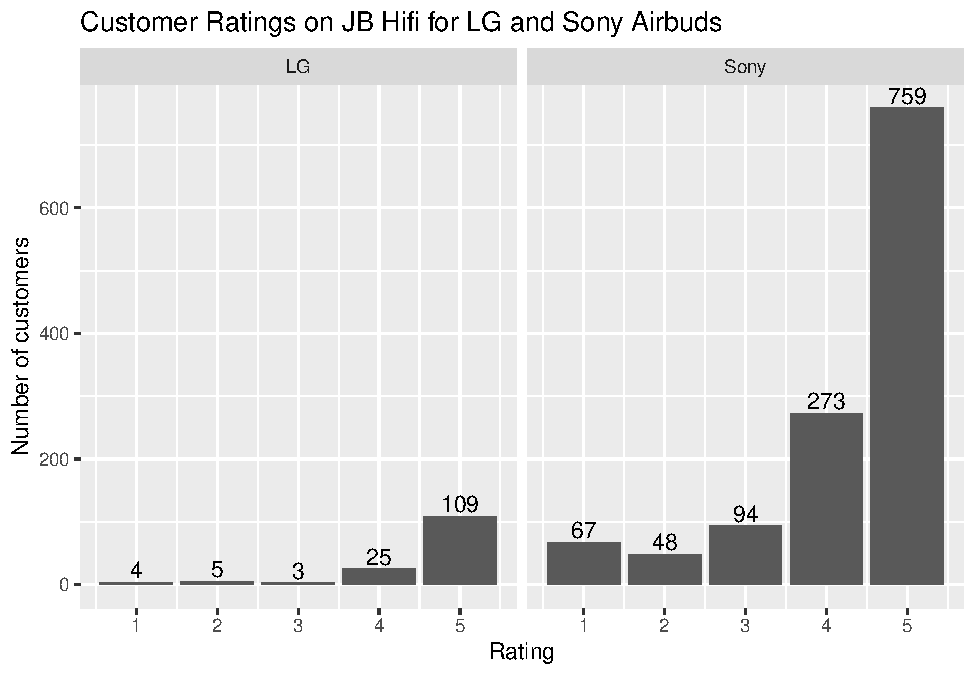
\includegraphics{notes_files/figure-latex/unnamed-chunk-6-1.pdf}

Some of their important statistics can also be calculated:

\begin{Shaded}
\begin{Highlighting}[]
\NormalTok{alpha }\OtherTok{\textless{}{-}} \FloatTok{0.05}
\NormalTok{n\_lg }\OtherTok{\textless{}{-}} \FunctionTok{sum}\NormalTok{(earphones}\SpecialCharTok{$}\NormalTok{LG)}
\NormalTok{n\_sony }\OtherTok{\textless{}{-}} \FunctionTok{sum}\NormalTok{(earphones}\SpecialCharTok{$}\NormalTok{Sony)}

\NormalTok{averages }\OtherTok{\textless{}{-}}\NormalTok{ earphones }\SpecialCharTok{\%\textgreater{}\%} \FunctionTok{summarise\_at}\NormalTok{(}\FunctionTok{c}\NormalTok{(}\StringTok{"Sony"}\NormalTok{,}\StringTok{"LG"}\NormalTok{), }\FunctionTok{funs}\NormalTok{(}\AttributeTok{average =} \FunctionTok{sum}\NormalTok{(Ratings}\SpecialCharTok{*}\NormalTok{.)}\SpecialCharTok{/}\FunctionTok{sum}\NormalTok{(.)))}
\end{Highlighting}
\end{Shaded}

\begin{verbatim}
## Warning: `funs()` was deprecated in dplyr 0.8.0.
## Please use a list of either functions or lambdas: 
## 
##   # Simple named list: 
##   list(mean = mean, median = median)
## 
##   # Auto named with `tibble::lst()`: 
##   tibble::lst(mean, median)
## 
##   # Using lambdas
##   list(~ mean(., trim = .2), ~ median(., na.rm = TRUE))
## This warning is displayed once every 8 hours.
## Call `lifecycle::last_lifecycle_warnings()` to see where this warning was generated.
\end{verbatim}

\begin{Shaded}
\begin{Highlighting}[]
\NormalTok{lg\_bar }\OtherTok{\textless{}{-}}\NormalTok{ averages}\SpecialCharTok{$}\NormalTok{LG\_average}
\NormalTok{lg\_s }\OtherTok{\textless{}{-}} \FunctionTok{sum}\NormalTok{((earphones}\SpecialCharTok{$}\NormalTok{Ratings }\SpecialCharTok{{-}}\NormalTok{ lg\_bar)}\SpecialCharTok{\^{}}\DecValTok{2} \SpecialCharTok{*}\NormalTok{ earphones}\SpecialCharTok{$}\NormalTok{LG) }\SpecialCharTok{/}\NormalTok{ (}\FunctionTok{sum}\NormalTok{(earphones}\SpecialCharTok{$}\NormalTok{LG) }\SpecialCharTok{{-}} \DecValTok{1}\NormalTok{)}

\NormalTok{sony\_bar }\OtherTok{\textless{}{-}}\NormalTok{averages}\SpecialCharTok{$}\NormalTok{Sony\_average}
\NormalTok{sony\_s }\OtherTok{\textless{}{-}} \FunctionTok{sum}\NormalTok{((earphones}\SpecialCharTok{$}\NormalTok{Ratings }\SpecialCharTok{{-}}\NormalTok{ sony\_bar)}\SpecialCharTok{\^{}}\DecValTok{2} \SpecialCharTok{*}\NormalTok{ earphones}\SpecialCharTok{$}\NormalTok{Sony) }\SpecialCharTok{/}\NormalTok{ (}\FunctionTok{sum}\NormalTok{(earphones}\SpecialCharTok{$}\NormalTok{Sony) }\SpecialCharTok{{-}} \DecValTok{1}\NormalTok{)}

\NormalTok{Z\_critical }\OtherTok{\textless{}{-}} \FunctionTok{qnorm}\NormalTok{(}\DecValTok{1} \SpecialCharTok{{-}}\NormalTok{ alpha)}
\FunctionTok{cat}\NormalTok{(}\StringTok{"LG Size:}\SpecialCharTok{\textbackslash{}t}\StringTok{"}\NormalTok{, n\_lg, }\StringTok{"}\SpecialCharTok{\textbackslash{}n}\StringTok{"}\NormalTok{)}
\end{Highlighting}
\end{Shaded}

\begin{verbatim}
## LG Size:  146
\end{verbatim}

\begin{Shaded}
\begin{Highlighting}[]
\FunctionTok{cat}\NormalTok{(}\StringTok{"LG Average:}\SpecialCharTok{\textbackslash{}t}\StringTok{"}\NormalTok{, lg\_bar, }\StringTok{"}\SpecialCharTok{\textbackslash{}n}\StringTok{"}\NormalTok{)}
\end{Highlighting}
\end{Shaded}

\begin{verbatim}
## LG Average:   4.575342
\end{verbatim}

\begin{Shaded}
\begin{Highlighting}[]
\FunctionTok{cat}\NormalTok{(}\StringTok{"LG sd:}\SpecialCharTok{\textbackslash{}t\textbackslash{}t}\StringTok{"}\NormalTok{, lg\_s, }\StringTok{"}\SpecialCharTok{\textbackslash{}n}\StringTok{"}\NormalTok{)}
\end{Highlighting}
\end{Shaded}

\begin{verbatim}
## LG sd:        0.8253188
\end{verbatim}

\begin{Shaded}
\begin{Highlighting}[]
\FunctionTok{cat}\NormalTok{(}\StringTok{"Sony Size:}\SpecialCharTok{\textbackslash{}t}\StringTok{"}\NormalTok{, n\_sony, }\StringTok{"}\SpecialCharTok{\textbackslash{}n}\StringTok{"}\NormalTok{)}
\end{Highlighting}
\end{Shaded}

\begin{verbatim}
## Sony Size:    1241
\end{verbatim}

\begin{Shaded}
\begin{Highlighting}[]
\FunctionTok{cat}\NormalTok{(}\StringTok{"Sony Average:}\SpecialCharTok{\textbackslash{}t}\StringTok{"}\NormalTok{, sony\_bar, }\StringTok{"}\SpecialCharTok{\textbackslash{}n}\StringTok{"}\NormalTok{)}
\end{Highlighting}
\end{Shaded}

\begin{verbatim}
## Sony Average:     4.296535
\end{verbatim}

\begin{Shaded}
\begin{Highlighting}[]
\FunctionTok{cat}\NormalTok{(}\StringTok{"Sony sd:}\SpecialCharTok{\textbackslash{}t}\StringTok{"}\NormalTok{, sony\_s, }\StringTok{"}\SpecialCharTok{\textbackslash{}n}\StringTok{"}\NormalTok{)}
\end{Highlighting}
\end{Shaded}

\begin{verbatim}
## Sony sd:  1.241028
\end{verbatim}

Which one would you pick?

We all lean towards the Sony one with more ratings, but lower average.

\textbf{Go to www.menti.com and use the code 2380 3183}

\hypertarget{are-they-both-good}{%
\paragraph{Are they both good?}\label{are-they-both-good}}

It is generally believed that a good product should have an average
rating of at least 4.25 (or 85\%). Given the reviews above, is there
enough evidence to conclude that both Airbuds are good products, given a
Type I error rate of 0.05?

Since we want to find if a product has greater than or at least 4.25
stars on average. This should be our alternate hypothesis.

\[
H_A = \mu \geq 4.25
\]

That means our null hypothesis is:

\[
H_0 = \mu < 4.25
\]

For a type I error rate of \(\alpha = 0.05\), the critical value is:

\begin{Shaded}
\begin{Highlighting}[]
\NormalTok{alpha }\OtherTok{\textless{}{-}} \FloatTok{0.05}
\NormalTok{Z\_critical }\OtherTok{\textless{}{-}} \FunctionTok{qnorm}\NormalTok{(}\DecValTok{1} \SpecialCharTok{{-}}\NormalTok{ alpha) }\CommentTok{\# Since this is a one sided test}
\NormalTok{Z\_critical}
\end{Highlighting}
\end{Shaded}

\begin{verbatim}
## [1] 1.644854
\end{verbatim}

\[
Z_{\alpha} = Z_{0.05} \approx 1.645
\]

Find the test statistics:

\begin{enumerate}
\def\labelenumi{\alph{enumi})}
\tightlist
\item
  For the Sony earbuds:
\end{enumerate}

Sony Size: 1241 Sony Average: 4.296535 Sony sd: 1.241028

\[
\begin{aligned}
n &= 1241\\
\bar{x} &= 4.297\\
s &= 1.241\\
\mu_0 &= 4.25 \\
Z &= \dfrac{\bar{x} - \mu_0}{s/\sqrt{n}}\\
&= \dfrac{4.297 - 4.25}{1.241/\sqrt{1241}}\\
&= 1.334
\end{aligned}
\]

Check if test statistics is greater than critical statistics (because
the null hypothesis has the form \(H_0: \mu \leq \mu_0\).

\[
Z > Z_{\alpha}?\\
Z = 1.334 < 1.645
\]

This means our test statistics does not pass the test. We fail to reject
the null hypothesis.

Alternately, we say that the Sony earbuds may not be a good product.

\begin{Shaded}
\begin{Highlighting}[]
\NormalTok{(}\FloatTok{4.297} \SpecialCharTok{{-}} \FloatTok{4.25}\NormalTok{)}\SpecialCharTok{/}\NormalTok{(}\FloatTok{1.241}\SpecialCharTok{/}\FunctionTok{sqrt}\NormalTok{(}\DecValTok{1241}\NormalTok{))}
\end{Highlighting}
\end{Shaded}

\begin{verbatim}
## [1] 1.334172
\end{verbatim}

\begin{enumerate}
\def\labelenumi{\alph{enumi})}
\setcounter{enumi}{1}
\tightlist
\item
  For the LG earbuds:
\end{enumerate}

LG Size: 146 LG Average: 4.575342 LG sd: 0.8253188

\[
\begin{aligned}
n &= 146\\
\bar{x} &= 4.575\\
s&= 0.825\\
\mu_0 &= 4.25\\
Z_\alpha &= 1.645\\
Z &= \dfrac{\bar{x} - \mu_0}{s/\sqrt{n}}\\
&= \dfrac{4.575 - 4.25}{0.825/\sqrt{146}}\\
&\approx 4.760 > Z_{\alpha}
\end{aligned}
\]

We reject the null hypothesis and accept that the LG earbuds is a good
product.

\begin{Shaded}
\begin{Highlighting}[]
\NormalTok{(}\FloatTok{4.575} \SpecialCharTok{{-}} \FloatTok{4.25}\NormalTok{) }\SpecialCharTok{/}\NormalTok{ (}\FloatTok{0.825}\SpecialCharTok{/}\FunctionTok{sqrt}\NormalTok{(}\DecValTok{146}\NormalTok{))}
\end{Highlighting}
\end{Shaded}

\begin{verbatim}
## [1] 4.759988
\end{verbatim}

\hypertarget{which-pair-is-better-statistically}{%
\paragraph{Which pair is better,
statistically?}\label{which-pair-is-better-statistically}}

Perform a test to check if the LG buds are statistically better than the
Sony buds.

Define our alternate hypothesis as:

\[
H_A: \mu_{LG} > \mu_{Sony}\\
H_A: \mu_{LG} - \mu_{Sony} > 0
\]

That means our null hypothesis is:

\[
H_0: \mu_{LG} - \mu_{Sony} \leq 0
\]

This is a one sided test.

LG Size: 146 LG Average: 4.575342 LG sd: 0.8253188 Sony Size: 1241 Sony
Average: 4.296535 Sony sd: 1.241028

\[
\begin{aligned}
\Delta_0 &= 0 \\
\bar{x_{lg}} &=  4.575\\
s_{lg} &= 0.825\\
n_{lg} &= 146\\
\bar{x_{sony}} &= 4.297\\
s_{sony} &= 1.241\\
n_{sony} &= 1241\\
\end{aligned}
\]

Since \(\alpha = 0.05\), the critical Z score is the same as above:

\[
Z_\alpha = 1.645
\]

\[
\begin{aligned}
Z &= \dfrac{(\bar{x_{lg}} - \bar{x_{sony}})-\Delta_0}{\sqrt{\dfrac{s_{lg}^2}{n_{lg}}+\dfrac{s_{sony}^2}{n_{sony}}}}\\
&= \dfrac{(4.575 - 4.297) - 0}{\sqrt{\dfrac{0.825^2}{146}+\dfrac{1.241^2}{1241}}}\\
&\approx 3.618
\end{aligned}
\]

\begin{Shaded}
\begin{Highlighting}[]
\NormalTok{num }\OtherTok{\textless{}{-}} \FloatTok{4.575} \SpecialCharTok{{-}} \FloatTok{4.297}
\NormalTok{den }\OtherTok{\textless{}{-}} \FunctionTok{sqrt}\NormalTok{(}\FloatTok{0.825}\SpecialCharTok{\^{}}\DecValTok{2}\SpecialCharTok{/}\DecValTok{146} \SpecialCharTok{+} \FloatTok{1.241}\SpecialCharTok{\^{}}\DecValTok{2}\SpecialCharTok{/}\DecValTok{1241}\NormalTok{)}
\NormalTok{num}\SpecialCharTok{/}\NormalTok{den}
\end{Highlighting}
\end{Shaded}

\begin{verbatim}
## [1] 3.618389
\end{verbatim}

Test if the test statistics is greater than the critical statistic
(\(Z_{\alpha} = 1.645\)).

\[
Z > Z_\alpha\\
\text{since}\\
3.618 > 1.645
\]

Hence, we reject the null hypothesis and conclude that the LG buds are
better than the Sony buds in terms of ratings.

\hypertarget{workshop-9-41022}{%
\subsection{Workshop 9 (4/10/22)}\label{workshop-9-41022}}

\hypertarget{workshop-10-111022}{%
\subsection{Workshop 10 (11/10/22)}\label{workshop-10-111022}}

\hypertarget{workshop-11-181022}{%
\subsection{Workshop 11 (18/10/22)}\label{workshop-11-181022}}

\hypertarget{workshop-12-231022}{%
\subsection{Workshop 12 (23/10/22)}\label{workshop-12-231022}}

\end{document}
